\documentclass[12pt]{report}
\usepackage[utf8]{inputenc}
\usepackage[frenchb]{babel}
\usepackage[official]{eurosym}
\usepackage{amsmath}
\usepackage{graphicx}
\usepackage{wrapfig}
%\DeclareGraphicsExtensions{.pdf,.png,.jpg,.eps}%
\begin{document}

%\includegraphics{elecshock}%

\title{Transmission d'electricité sans fil par le biais de systemes de tranfert d'energie inductive (IPTS)}
\author{Blaise Ribon, Léo Boudoin, Quentin Boyer}
\date{Décembre 2014}
\maketitle

\begin{abstract}
	Suite a l'experience menée en 2007 au MIT , nous savons qu'il est possible de transmettre de l'electricité à travers de moyennes distances, de l'ordre de 5m. Ce type de transmissions d'electricité pourrait simplifier les reseaux electriques domestiques étant donné le nombre de cables demandés par chaque appareil electronique, qui proliferent. Mais nous verrons que cette technologie et celles semblables se heurtent à des freins majeurs dans la pratique et que leur mise en place est assez complexe.
\end{abstract}

\tableofcontents

\chapter{Définition et Utilisation de l'electricité} %Titre a changer je pense%
\section{Historique de l'electricité}

\begin{figure}[h!]
  \caption{Le feu dans la prehistoire}
  \centering
	\includegraphics[width=10cm]{feu_prehisoire}
\end{figure}

	    À la Préhistoire déjà, l'Homme a utilisé l'électricité. Par le biais de l'effet Joule, la foudre, en tombant sur le sol, pouvait enflammer des arbres, et parfois créer des incendies dévastateurs. En utilisant ces flammes, les hommes de cette époque on pu se procurer lumière et chaleur, ainsi qu'une protection efficace contre les prédateurs de l'époque, chose si rare et recherchée qu'elle a donné naissance au mythiques "guerres du feu". Là se résume l'histoire de la domestication de l'électricité pendant des millénaires.
\begin{wrapfigure}{r}{0.3\textwidth}
  \begin{center}
    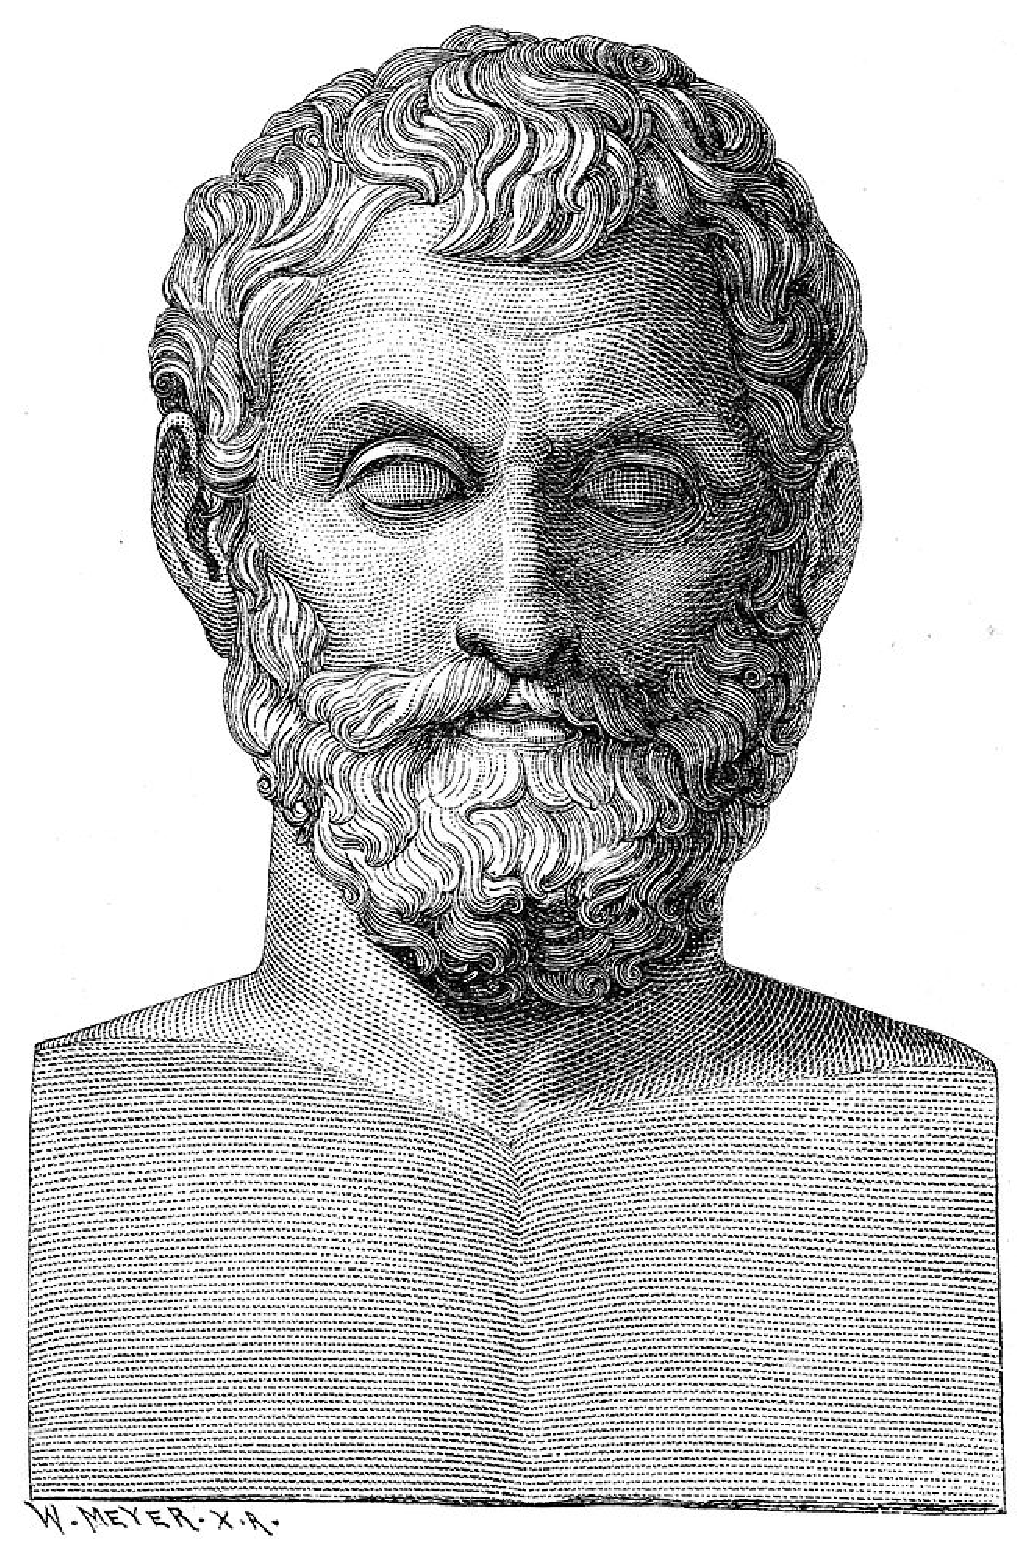
\includegraphics[width=0.225\textwidth]{thales}
  \end{center}
  \caption{Thales}
\end{wrapfigure} Jusqu'au jour où Thalès de Milet(vers 625-vers 547 anvant JC), un philosophe grec de l'Antiquité observe le fait que l'ambre jaune, frotté, attire des corps légers comme des brins de paille ou des barbes de plumes. Il baptisera ce phénomène du nom grec de l'ambre jaune, "elektron".

  Par la suite, ce mot servira à nommer l'électricité ou tous les phénomènes ayant un rapport. Par la suite, les découvertes se sont succédées lentement juqu'au XVIIIe siècle. On pourra citer la première machine à éléctricté statique d'Otto Von Guericke(1602-1686), constitué d'un simple globe de soufre, ou la classification des corps en fonction de leur comportement, idio-électriques(isolants), et anélectriques(conducteurs), par William Gilbert(1544-1600), et est le premier à relier électricité et magnétisme.

    Dès 1709 les découvertes s'accélèrent. Francis Hawskbee remplece le globe de soufre de Von Guericke par un cylindre en verre en 1709, et Stephen Grey découvre par hasard que les charges produites par la machine de Hawksbee se déplacent vers le bouchon. Cela amènera, plus tard à la découverte de la portée infinie des charges électriques le long d'un conducteur, avec l'aide de Charles François de Cisternay du Fay. Il découvre aussi que le corps humain est conducteur, et définit deux types d'électricité: la "résineuse"(quand de la résine est frottée) et la "vitreuse"(quand du verre est frotté), qui prépare la découverte de la charge de signes opposés. il créera aussi le premier electroscope connu.

\begin{wrapfigure}{r}{0.45\textwidth}
  \begin{center}
    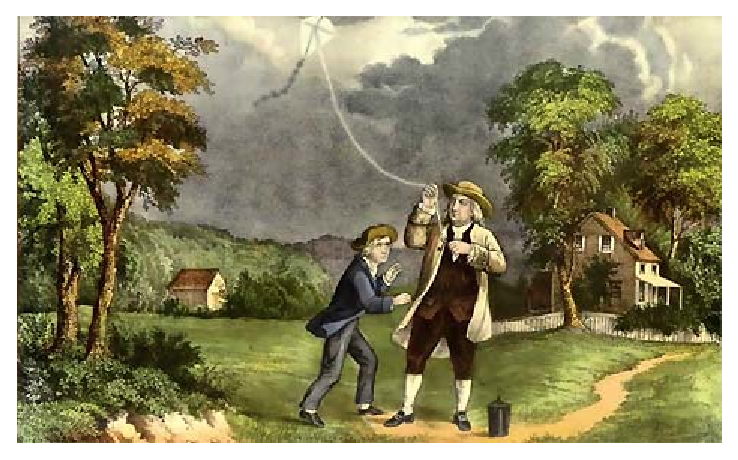
\includegraphics[width=0.4\textwidth]{franklin}
  \end{center}
  \caption{Franklin}
\end{wrapfigure}
De nombreuses autres découvertes ont été faites durant ce siècle, comme les travaux de Benjamin Franklin (1706-1790) avec la mythique expérience où ce scientifique a sorti un cerf-volant sous un orage(à ne pas reproduire) pour savoir "si les nuages d'où jaillit la foudre sont électrisés ou non", ce qui mènera à la découverte du paratonnerre. Plus tard, Alessandre Volta(1745-1827) multiplie les découvertes dans le domaine de l'électricité. Il crée et améliore de nombreux appareils de mesure électrique, met au point l'électrophore, capable d'accumuler de grandes charges électriques positives, et crée la preière pile. Charles de Coulomb(1736-1806) établira en 1785 la loi homonyme, quantifiant la force électrostatique. Elle définit la force qu'exercent deux charges l'une sur l'autre
\begin{wrapfigure}{l}{0.3\textwidth}
  \begin{center}
    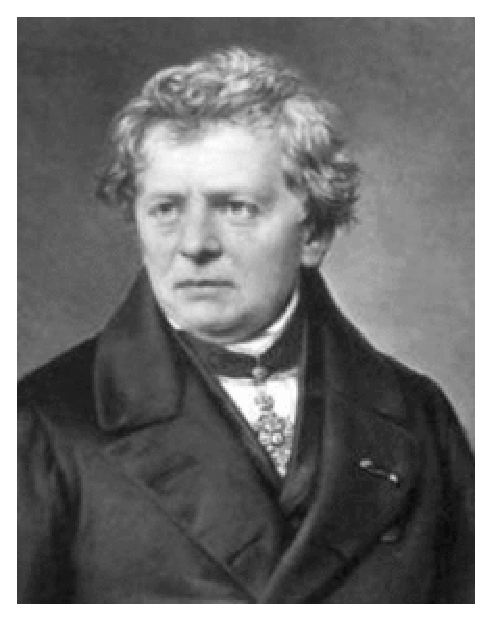
\includegraphics[width=0.25\textwidth]{ohm}
  \end{center}
  \caption{Ohm}
\end{wrapfigure}
 (\(\vec{F_{1/2}}=\frac{q1q2}{4\pi \varepsilon _{0}}\frac{\vec{r_{2}}-\vec{r_{1}}}{\| \vec{r_{2}}-\vec{r_{1}} \|  ^{3}} \), ou q1 et q2 sont en C, \(\varepsilon _{0}\) en \(F.m^{-1}\) et \(\vec{r_{1}}\) et \(\vec{r_{2}}\)
sont des points). Elle est attractive si les chragessont de signe contraire, et répulsive si les charges sont de même signe. Au XIXe siècle, la recherche s'accélère encore. Au début du siècle, sir Humphrey Davy(1778-1829) étudie et met au point la première pile à combustible. Sous la férule de Faraday, il créera aussi la première source de lumière électrique, l'arc électrique. En même temps, Georg Simon Ohm(1787-1854), découvre la résistance des conducturs et etudie les propriétés quantitatives des courants électriques, dont il formule les lois fondamentales. La loi d'Ohm est une relation simple entre l'intesnité, la tension, et la résistance \( I = U \times R \) , avec I pour l'intensité, en ampères, U pour les tension, en volts, et R pour la résistance, en Ohms.
    
    En découvrant cette propriété, il affine la notion d'électricité suffisamment pour la rendre utilisable, et ce sera sur cet axe que la recherche scientifique sera axée dès le second quart du siècle.
\section{Avancées technologiques et Utilisation}

\chapter{Raisons de la transmission de l'electricité par des solutions non cablées} %Titre encore plus pété , Mais en fait on pourrait faire la demarche de projet sur la transimission d'electicté tout court en preseantant tour a tour les solutions cablées et non cablées , à voir%
\section{--TODO--}

\chapter{Les technologies de transmissions d'electricité : cablées et sans-fil} %A voir si on insiste autant sur les cables%
\section{Presentation des technologies présentes}
\subsection{Solution majoritaire actuelle : Les technoloogies cablées}
\begin{wrapfigure}{r}{0.4\textwidth}
  \begin{center}
    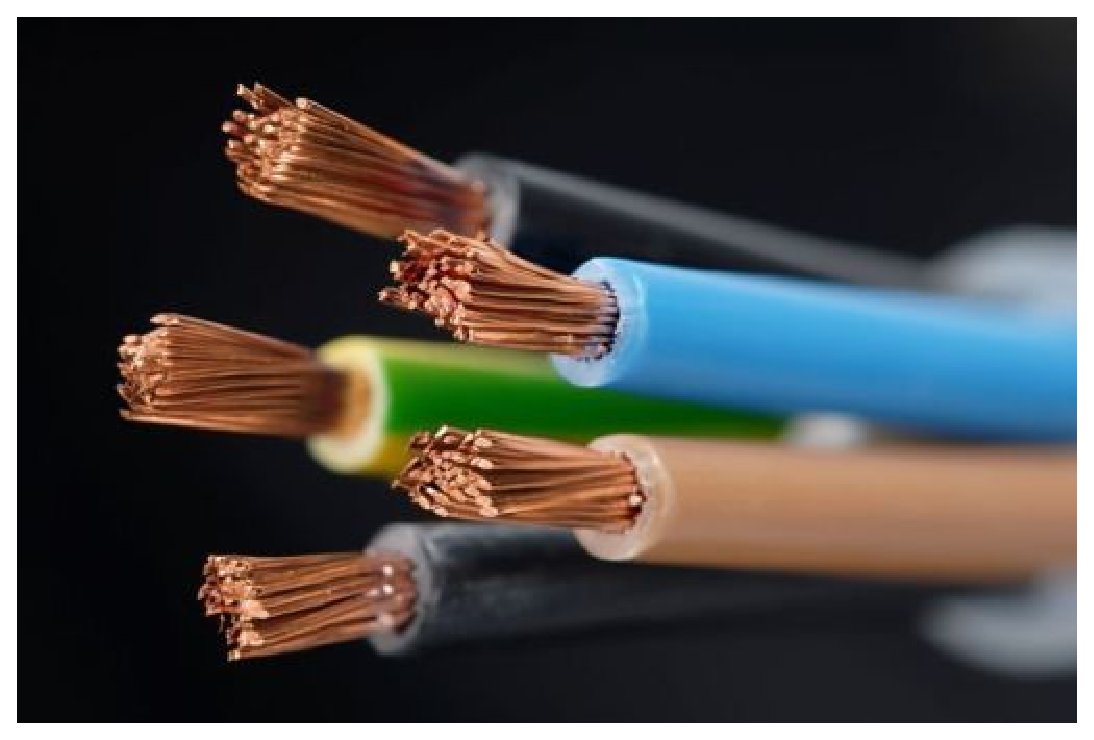
\includegraphics[width=0.3\textwidth]{copperWire}
  \end{center}
  \caption{Fils du cuivres}
\end{wrapfigure} La solution de transmission d'electricité la plus utilisée au monde est sans contestation possible le cable electrique , ceci étant du à un faible coût (jusqu'a 1\$ le métre) , son très haut rendement puisque celui ci avoisine les 100\% sur les distances courtes avec de faibles puissances. En plus d'etre simple , elle n'est pas lourde en terme d'installation puisque les cables peuvent etre facilement mis dans les murs à la constuction d'un nouveau batiment, etre mis dans des gaines si l'on veut en rajouter ensuite et plus simplement on peut utiliser le systeme des prises pour les appareils temporaires et ponctuels. Grâce à ses avantages incontesables elle est devenue le standard , mais ceci entraîne un probleme non negligable qu'es la densité importante des cables electriques à proximité des appareils electroniques.
	
	Les matériau consituant les cables electriques sont generalement du cuivre pour les longues distances, mais dans les circuitis imprimé on peut utiliser l'or pour sa conductivité electrique immense , malgré son coût monstreux de l'ordre de la dizaine de millier d'euros le demi kilo. Voici ici un tableau qui récapitule la conductivité de divers métaux plus ou moins utilisés dans les réseaux cablées.

\begin{center}
\begin{tabular}{| l | c | r |}
	\hline
	Materiel & Resistivité électrique en \( n\Omega .m \)& Prix au Kilo \\
	\hline
	Cuivre & 16.78 & 1.08 \euro{}  \\
	Or & 22.14 & 29878 \euro{}  \\
	Fer & 96.1 & (Minerai de fer) 0.07 \euro{}  \\
	Argent & 15.87 & 402 \euro{}  \\
	\hline
\end{tabular}
\end{center}

\begin{wrapfigure}{l}{0.5\textwidth}
  \begin{center}
    \setlength\fboxsep{0pt}
    \setlength\fboxrule{0.5pt}
    \fbox{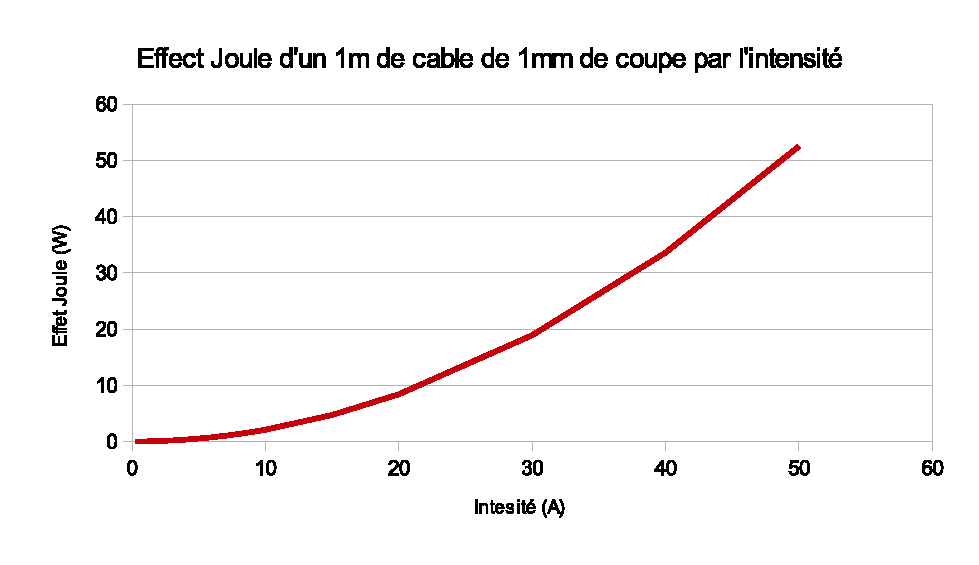
\includegraphics[width=0.45\textwidth]{Joule}}
  \end{center}
  \caption{L'effet joule}
\end{wrapfigure}Un effet négatif important produit par des cables est l'effet Joule , exprimé dans dans le cadre d'application de la loi d'Ohm par la formule \( P=I^{2} \times R\) ou R est la resitance est liée a la resistivité (\(\rho\)) par la formule \( R= \rho \frac{\ell}{A} \) dans laquelle \(\ell\) est la longeur et A est la surface de coupe en \(m^2\).
D'ou la resistance d'un cable de 1m de long et de 1mm de diamétre est \(17 \times 10^{-9} \times \frac{1}{\pi (0.5 \times 10^{-3})^{2}} = 0.021 \Omega \) et donc l'effect joule produit dans le cas d'un courant de 1A est de \( P=1^{2} \times 0.02 = 0.02 W\).

	Néamoins d'autres problemes peuvent occurer dans le cas d'une utilisation domstique , comme la profusion de cable qui genrent des nuisances esthetiques et des nuisances magnétiques générés par les cables nombreux qui subissent le phenomene de diaphonie (ou crosstalk)
\begin{wrapfigure}{r}{0.4\textwidth}
  \begin{center}
    \setlength\fboxsep{0pt}
    \setlength\fboxrule{0.5pt}
    \fbox{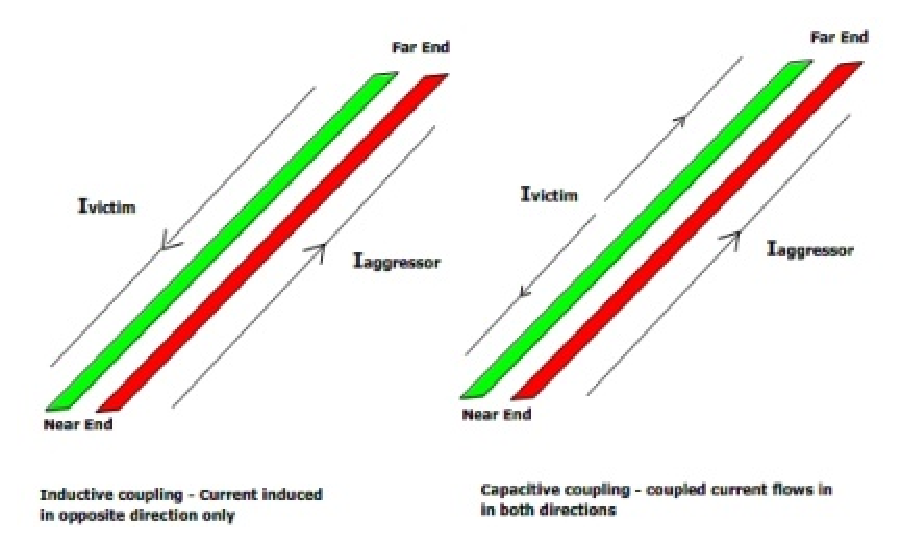
\includegraphics[width=0.3\textwidth]{crosstalk}}
  \end{center}
  \caption{Diaphonie}
\end{wrapfigure}, qui est une interfernce entre les signaux passant par un cable dans un cable proche. C'est d'ailleur pour cette raison que lorsque les signaux transmis sont importants et ne doivent pas etre corompus on utilise des cables torsadés qui limite le phenomene. La problematique du transport d'objets electroniques de plus en plus consomateurs mais qui se veulent autonomes se pose , ou l'on est obligé de se separer d'eux pour les recharger ceic emepechant de benficier des avantages majeurs de ces objets autonomes , avec comme exemple le cas des telephones portables , ou la problematique plus importante du rehcargement des voitures electriques qui est long , et qu'il ne faut pas oublier de brancher un cable sinon rien n'occure. Les cables electriques que nous utilisons donc depuis la création de l'electricité ne sont plus adapté a un monde qui se veut de plus en plus liberé de toute les contraintes et de s'affranchir des contraites liés au tehcnolgies filiares , avec comme exemple le devloppement des telephones portables ou 
de la wifi pour pallier la dependance cablée de l'ethernet.

\subsection{Une solution IPTS efficace : Le systeme de couplage magnetique par resonnace (CMRS) \cite{mSojal}}
\begin{wrapfigure}{r}{0.5\textwidth}
  \begin{center}
  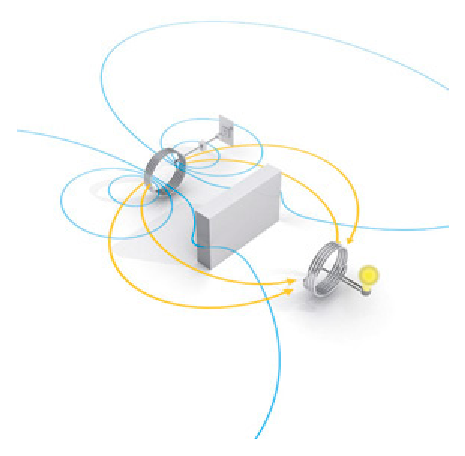
\includegraphics[width=0.4\textwidth]{WTdiagram}
  \end{center}
\caption{Diagramme}
\end{wrapfigure}Le MIT , par l'equipe de Marin Soljačić , a developé en 2007 une technolgie inductive utlisant le meme pricipe que les transfomateurs electetriques ou les brosses a dent eletriques. Mais en utilisant des variations de cette tehnologies cette equipe du MIT a reussi a transmettre de l'energie a une television située de l'autre coté de la piece , assez pour l'alimenter. Mais le probleme de cette technologie est qu'elle est extremement dépendante de l'envitonement , une petite variation tel le passage d'un etre humain , un autre champ magnetique qui perturbe les syteme ou une variation de la temperature ou de l'humidité peut invalider l'experience. Cette technologie a aussi un incovenient majeur, partagé par tout les systemes inducifs de tranferts d'energie , plus souvents abregé en IPTS , qui est le rendement grandement inférieur à un cable éléctrique déployé sur la meme distance. Ceci est du a la nature meme de la technolige qui est un champ magnetique non ou peu dirigé contrairement a un cable electrique ou les eletrons n'ont que une suele direction possible pour traverser d'un bout a l'autre du systeme de transmission d'electricté. Néamoins cette technologie est basée sur la maximisation du rendement possbile par un systeme IPTS.

	La dependance au conditions est du au systeme meme : il exploite la resonnace magnétique des matériaux , c'est a dire la capacité du materiau a produire une réaction energetique lorsque'il est simulé par un champ magnétique particulier , et ce "champ magnetique de resonnance" est affecté par la temperature , et il est deformé par les obstacle tel qu'un humain. Cette depedance extreme au champ magnetique est du au tres haut facteur de qualité du systeme technique utilisés dans l'experience du MIT , qui ne laisse aucune marge d'erreur dans les frequences. De plus la mise en place des bobines utilisés pour transmetre de l'electricité demande des reglages plutot complexes ou les bobines doivent etre accordées pour reagir au bon champ magnetique.
	
\begin{wrapfigure}{l}{0.5\textwidth}
  \begin{center}
    \setlength\fboxsep{0pt}
    \setlength\fboxrule{0.5pt}
    \fbox{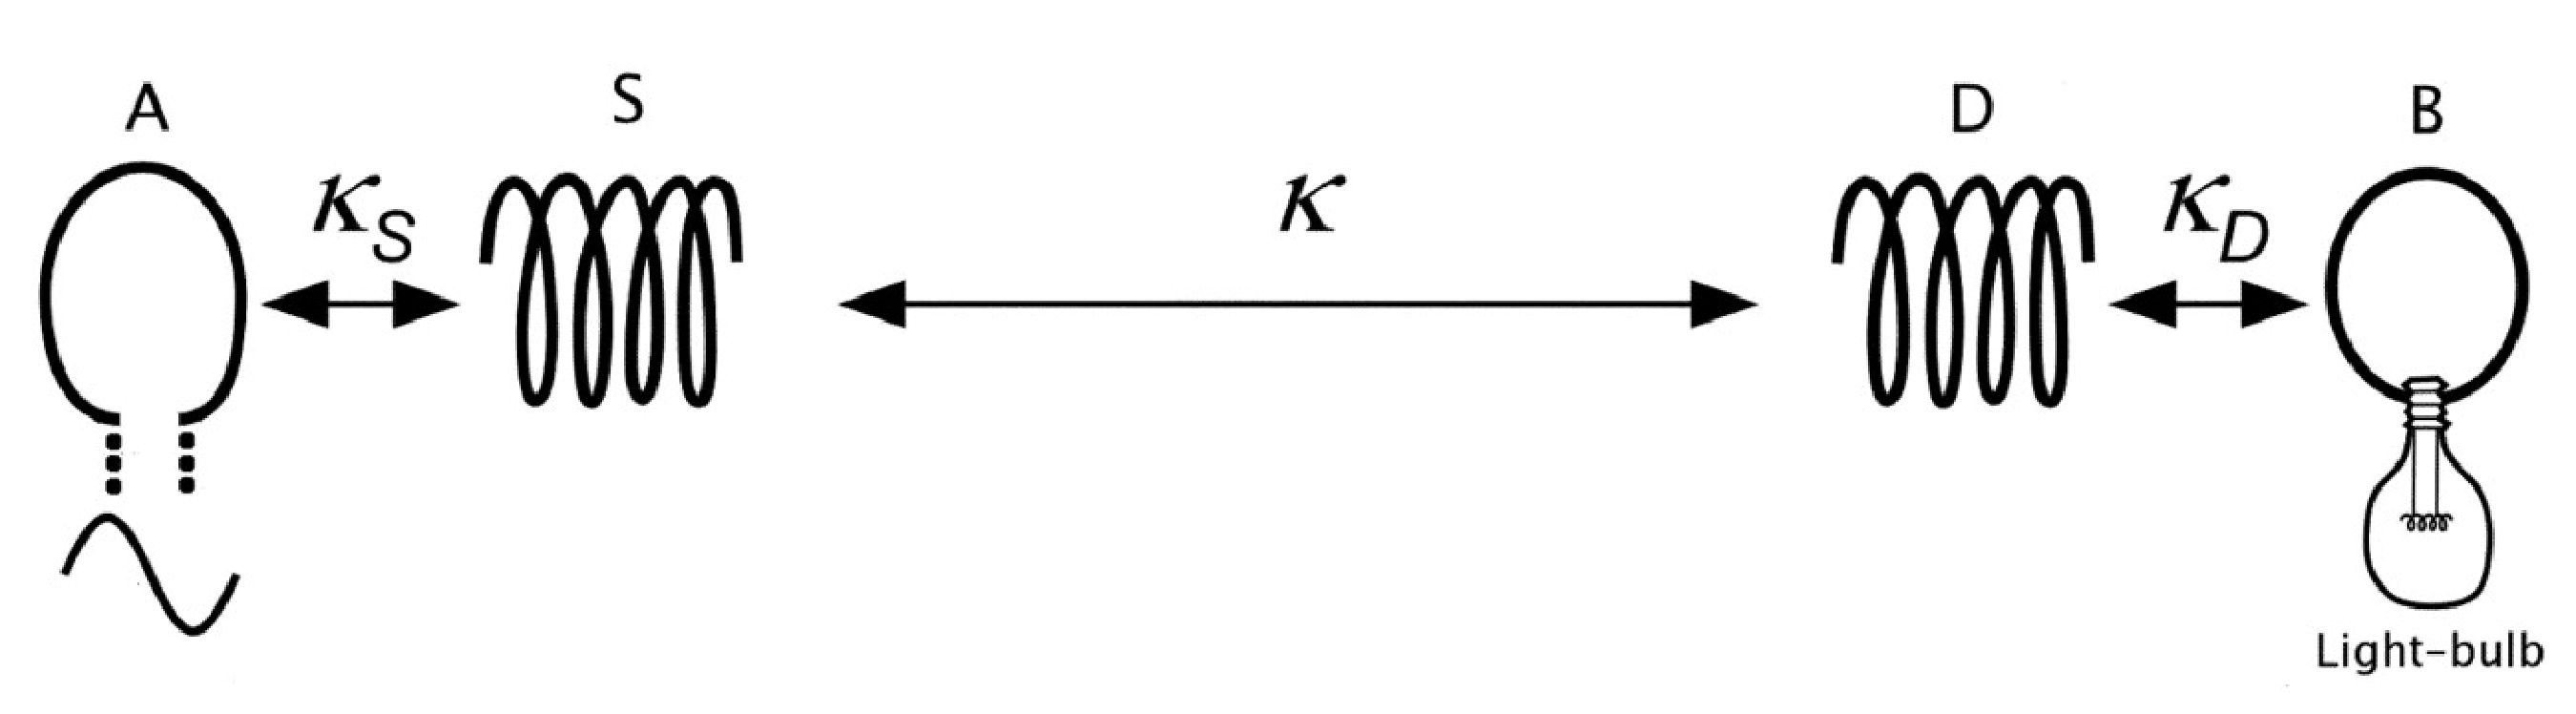
\includegraphics[width=0.45\textwidth]{cmrsMontage}}
  \end{center}
  \caption{Schema de montage}
\end{wrapfigure} Dans tout IPTS le principe fondamentale est identique : Le courant traversant une bobine de fil induit un courant proportionel dans une autre bobine. Dans la technologie ici présentée ces deux bobines doivent etre alignées coaxiallement. L'enrée et la sortie est effectuée via des boucles , et celle d'entrée A doit etre positionée de telle maniere qu'elle n'interfere pas avec la bobine D , l'influence de B sur S étant minimale.

  Cette technologie ne presente d'ailleurs que tres peu de danger \cite{wiki1} sur l'etre humain , étant donné que les champs magnetiques n'intergissant pratiquement pas avec les etre vivants , de meme que le reste de l'environement d'ou la ligne de vue entre les bobines S et D n'est pas nessecaire.
 D'apres Marin Soljačić cette technolgie à du potentiel puisque il a créé une compagnie , WiTricity , pour promulger sa découverte et il croit que cette technologie pourrait etre largement utilisé dans le cas de transfert de petites quantités d'energie comme recharger des telephones. 7 ans apres cette technologie ne s'est pas enormenet démocratisée meme si en 2011 Toyota a investi dans cette compagnie.
\subsection{Une solution IPTS assez fiable : Une transmission utilisant des \{Dipole coils\}\cite{kaist14}}
Contrairement au CMRS ou l'on pensait principalement à l'efficacité et au redement , faisant des bobines dependantes des conditions et plus adapté a transmettre des petites quantités d'energie , etant donné la complexité de la chose , les chercheurs du KAIST (Korea Advanced Institute of Science and Technology) en partenariat avec le departement nucléaire de corée ont developé une techlogie basée sur des \{Dipole coils\} qui est presque indépendante des conditions , grâce à un facteur qualité tres bas (\(\sim100\) , contrairement au CMRS qui avoisinait les 2000) et une technlogie plus simple a mettre en oeuvre , puisque la reponse n'est pas liée a des frequences tres specifiques , mais un peu plus larges.
  
  Cette technologie , étant soutenue par le departement nucléaire , à pour vocation de servir d'alimentation de secours dans le cadre de centrales nucléaires , ou le CMRS hyper-sensible ne convient pas , se veut a transmsetre des quantités d'energie largement supérieurs à celle prévue par Marin Soljačić. Pour pouvoir achever cet aspect la ils ont recourt a des frequences largement inférieurs au MIT qui utilisait du 9.9 MHz alors que le KAIST utilise des frequences de 20 kHz , qui est la raison de la baisse du facteur qualité.
  
\begin{wrapfigure}{r}{0.5\textwidth}
  \begin{center}
    \setlength\fboxsep{0pt}
    \setlength\fboxrule{0.5pt}
    \fbox{\includegraphics[width=0.4\textwidth]{coreenMontage}}
  \end{center}
  \caption{Montage}
\end{wrapfigure}Ici le syteme est consitués de deux barres de ferrite parraleles sur lesquelles sont enroulés 30 fois un fil , cette configuration étant due au peu de place disponible dans les centrales nucléaires et prends moins de place que le CMRS. Ces barres ont des dimension modulables proptionelement , tout comme le nombre de tours N. L'entrée est gerée par un \{Power Inverter\} et la sortie est presque utlisable telle que comme montré par le schema electrique qui suit.
\begin{figure}
  \begin{center}
    \includegraphics[width=7cm]{diagramC}
  \end{center}
  \caption{Diagramme}
\end{figure}

  Cette technologie est d'ailleurs beaucoup plus efficace lorsque l'on utilise de grande quantitées d'energie , étant donné que la puissance fournie n'est pas proptionnelle a l'intensité du systeme , mais accroit de plus en plus , comme montré par la figure 3.8. Ceci encore découle de la difference d'applications entre les deux technologies sans fils que nous avons présenté.
\begin{wrapfigure}{r}{0.3\textwidth}
  \begin{center}
    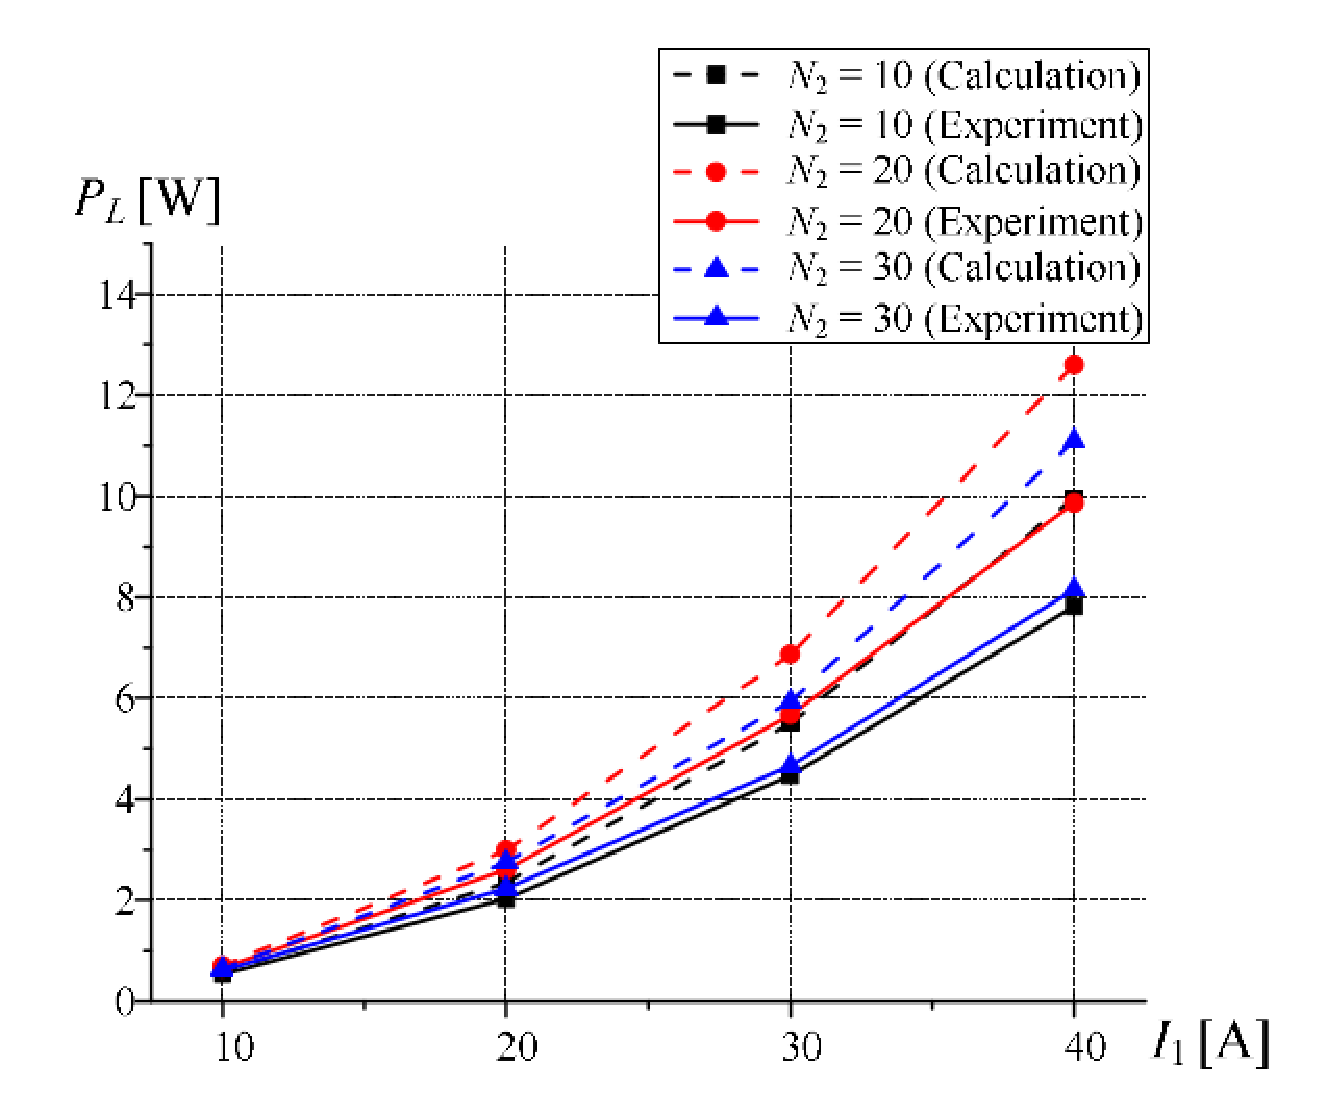
\includegraphics[width=0.2\textwidth]{PparI}
  \end{center}
  \caption{Puissance par intensité}
\end{wrapfigure}

  Contrairement au CMRS qui a eu le temps de se developper , cette technologie ayant été présentée en 2013 , elle n'a pas pu etre exploitée ni testée , et par consequent nous ne pouvons comparer completement objectivement ces deux technologies.
\section{Avantages et limitations des technologies étudiées}
\section{Technlogies alternatives pour transmetre de l'energie}
\begin{thebibliography}{9}
    
  \bibitem{mSojal}
  MIT,
  \emph{Wireless Power Transfer via Strongly Coupled Magnetic Resonances},
  2007.

  \bibitem{kaist14}
  KAIST,
  \emph{7m-off-Long-Distance Extremely Loosely Coupled Inductive Power Transfer Systems Using Dipole Coils},
  2014.
  
  \bibitem{wiki1}
  Wikipedia,
  \emph{Resonant inductive coupling}.
  
\end{thebibliography}
\end{document}
